\chapter{Results}

\section{Experimental Setup}

Our pipeline was evaluated on a dataset of images taken by us consisting
primarily of natural outdoor scenes with high spatial variance such as flowers, waterfalls, hills,
and architectural subjects. Images were processed at their native resolutions, with
$K = 3$ or $K = 4$ clusters used for segmentation depending on scene complexity.

\section{Qualitative Results}

Visual comparison of the original images against their enhanced output versoin
have demonstrated clear improvements across most test cases.
Figures below show that.

\begin{figure}[H]
    \centering
    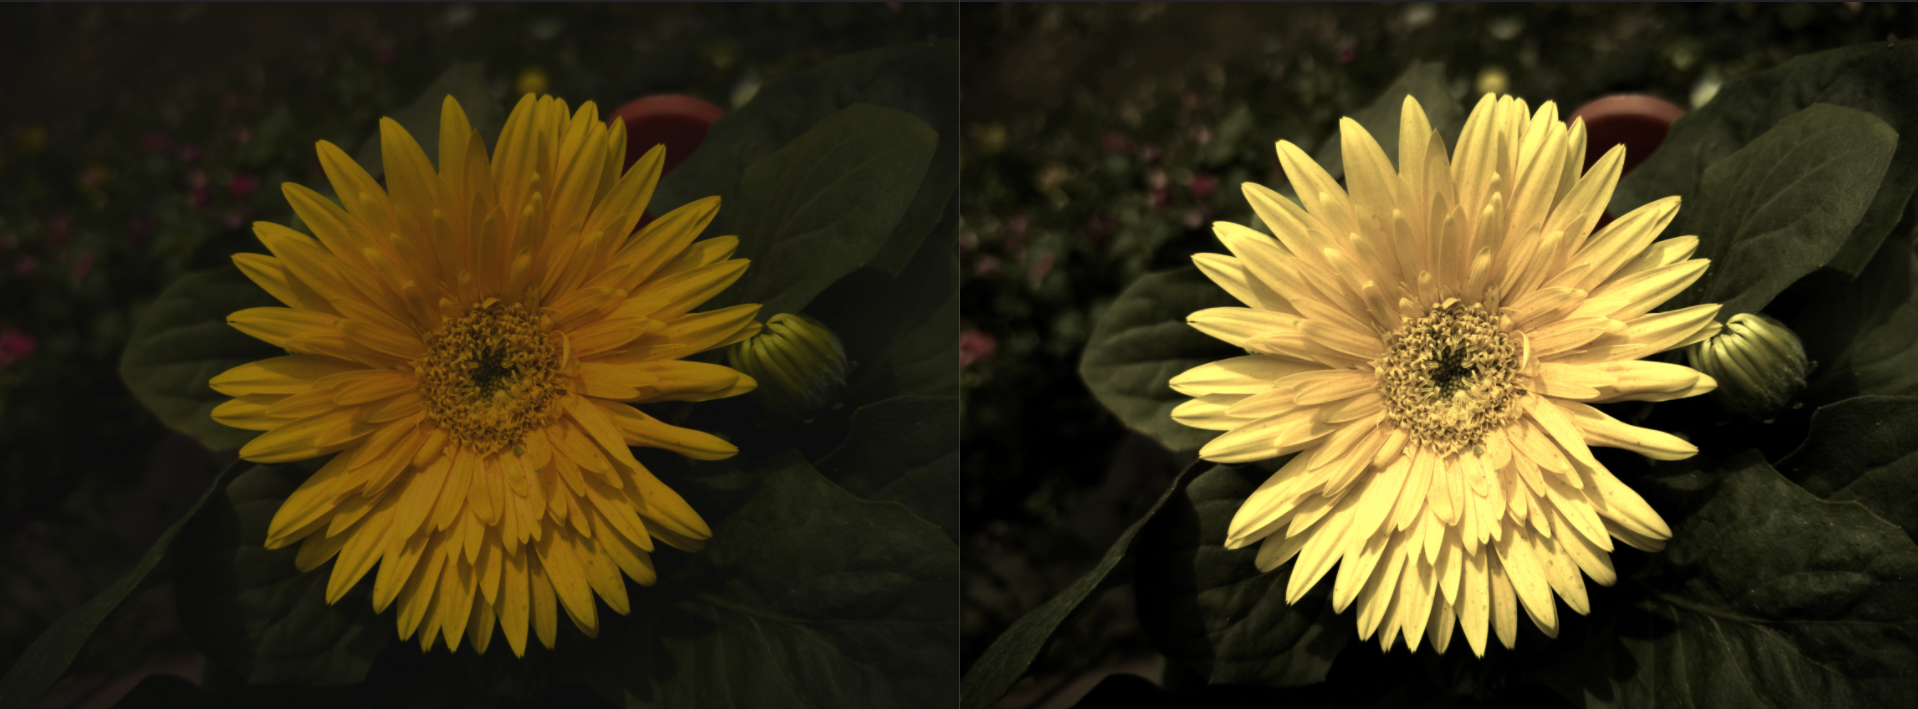
\includegraphics[width=\textwidth]{images/yellow-flower.png}
    \caption{Applying histogram stretching on the left image gives the enhanced image on the right(ouput)}
    \label{fig:placeholder}
\end{figure}
\begin{figure}[H]
    \centering
    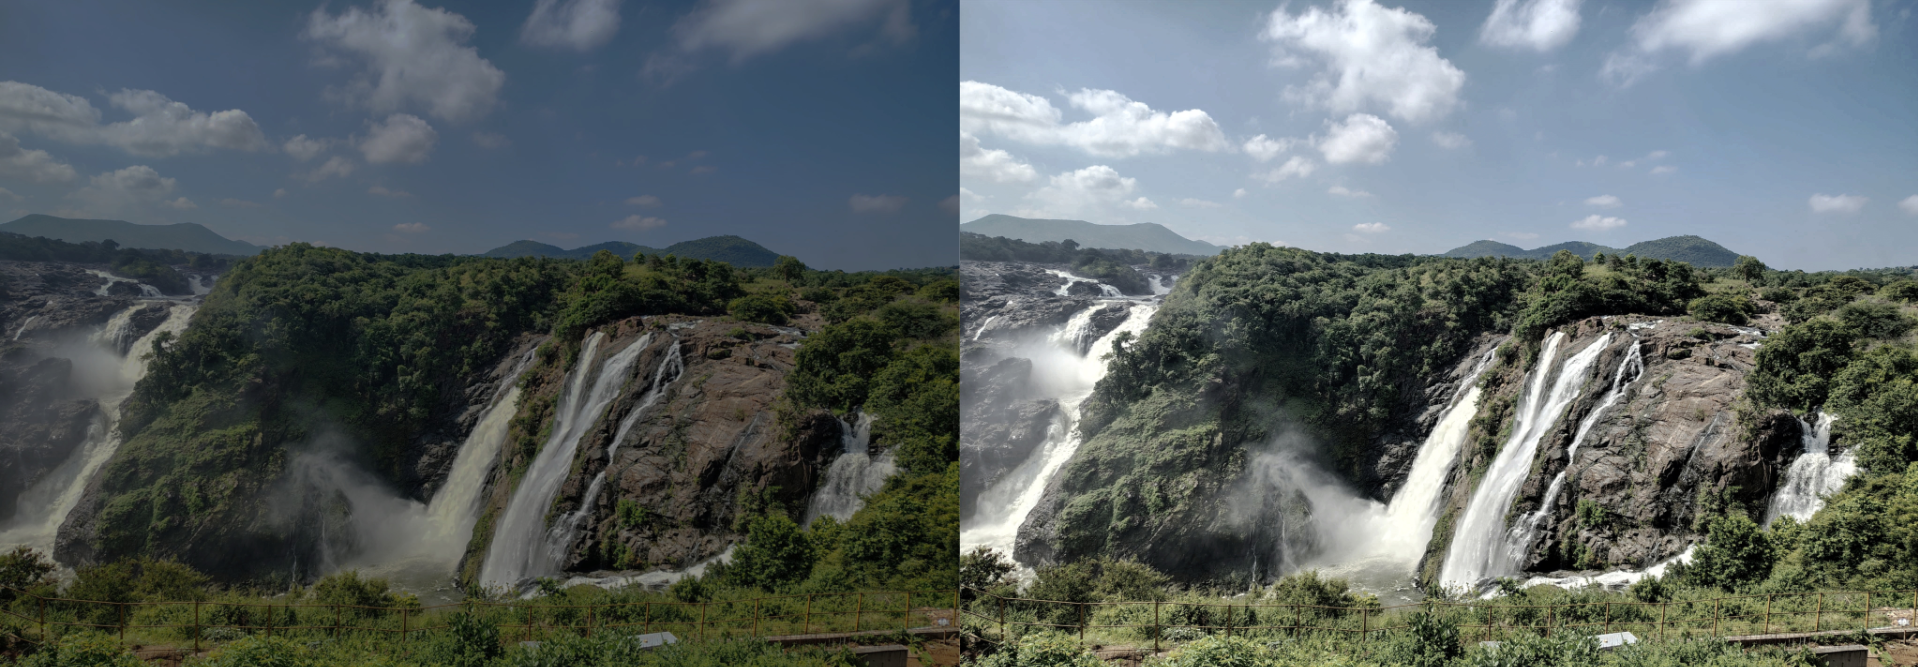
\includegraphics[width=\textwidth]{images/waterfall.png}
    \caption{Applying histogram stretching on the left image gives the enhanced image on the right(ouput)}
    \label{fig:placeholder}
\end{figure}


\begin{figure}[H]
    \centering
    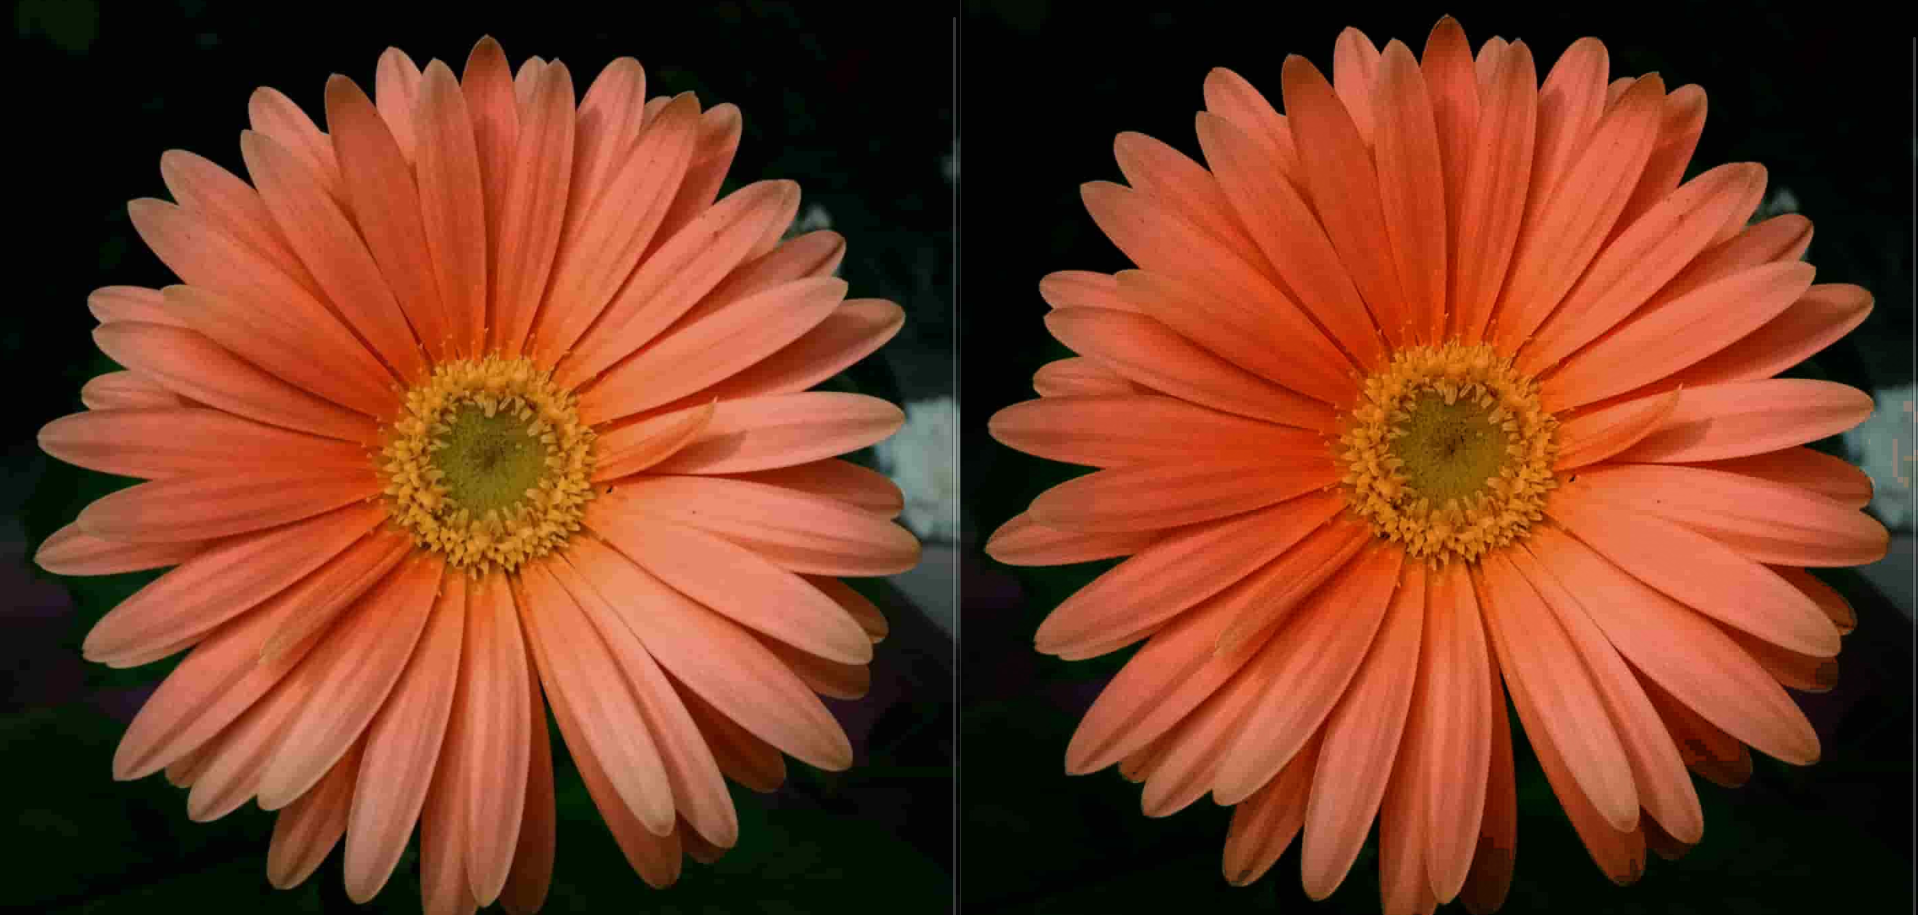
\includegraphics[width=\textwidth]{images/jpeg-blocks.png}
    \caption{Removal of JPEG blocks by inverse DCT. Left is input, right is ouput}
    \label{fig:placeholder}
\end{figure}


\begin{figure}[H]
    \centering
    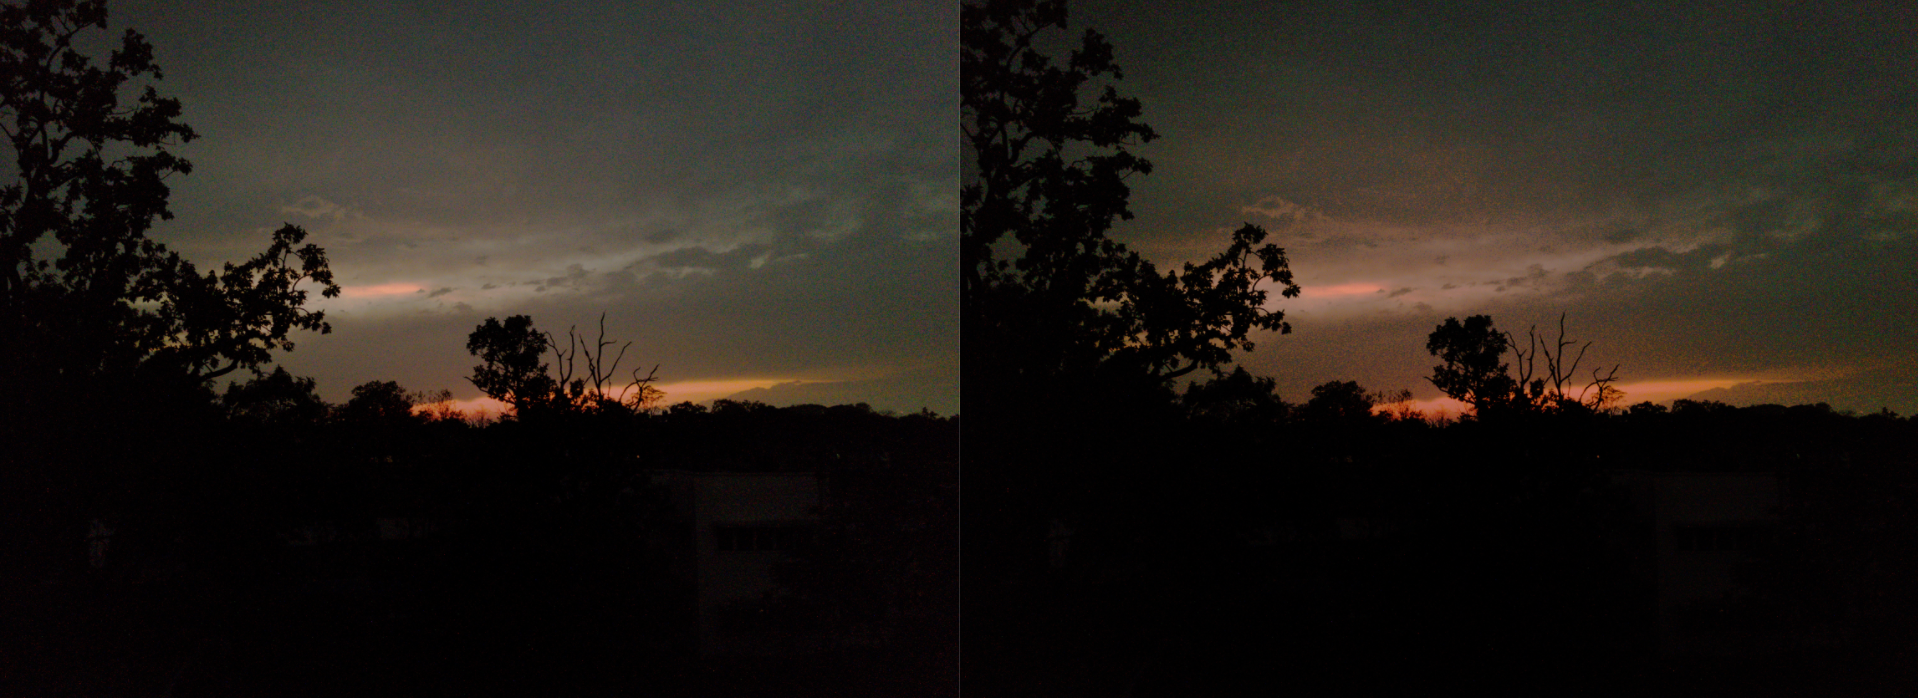
\includegraphics[width=\textwidth]{images/auto-enhancement.png}
    \caption{Original image (left) vs. auto-enhanced image (right)}
    \label{fig:placeholder}
\end{figure}

\begin{figure}[H]
    \centering
    \includegraphics[width=0.5\linewidth]{images/test6_segk4_overlay.jpg}
    \caption{k=4 segmentation for above example}
    \label{fig:placeholder}
\end{figure}

\section{Quantitative Evaluation}

\begin{figure}[H]
    \centering
    
\includegraphics[width=\textwidth]{images/eval.png}
    \label{fig:placeholder}
\end{figure}

Below are the results for image in fig.4.4

% --- Per-region metrics table ---
\begin{table}[H]
\centering
\caption{Per-region metrics (K=4 segmentation).}
\label{tab:region-metrics}
\begin{tabularx}{\textwidth}{l r c c c c c} 
\toprule
\textbf{Region} & \textbf{Pixels} & \textbf{Diagnosis} & \textbf{PSNR} & \textbf{SSIM} & \textbf{Entropy} & \textbf{Entropy} \\
& & & \textbf{(gray)} & \textbf{(gray)} & \textbf{Before} & \textbf{After} \\
\midrule
0 & ---       & Blurry & 22.867 dB & 0.894 & 5.934 & 5.942 (+0.009) \\
1 & 8,492,433 & Blurry & 38.921 dB & 0.850 & 3.239 & 2.568 ($-$0.671) \\
2 & 2,441,815 & Blurry & 24.104 dB & 0.882 & 5.739 & 5.802 (+0.063) \\
3 & 2,315,632 & Blurry & 26.396 dB & 0.972 & 6.301 & 6.496 (+0.194) \\
\midrule
\textbf{Summary} & --- & --- & \textbf{27.354 dB} & \textbf{0.946} & \textbf{5.660} & \textbf{5.354} \\
\bottomrule
\end{tabularx}
\end{table}

% --- Per-channel PSNR table ---
\begin{table}[H]
\centering
\caption{Per-channel PSNR (dB) by region.}
\label{tab:psnr-channels}
\begin{tabular}{lcccc}
\toprule
\textbf{Region} & \textbf{R} & \textbf{G} & \textbf{B} & \textbf{Grayscale} \\
\midrule
0       & 22.459 & 22.978 & 22.800 & 22.867 \\
1       & 36.222 & 39.099 & 38.040 & 38.921 \\
2       & 23.262 & 24.522 & 23.241 & 24.104 \\
3       & 35.064 & 23.114 & 22.612 & 26.396 \\
\midrule
\textbf{Summary} & \textbf{27.403} & \textbf{26.697} & \textbf{26.079} & \textbf{27.354} \\
\bottomrule
\end{tabular}
\end{table}

% --- Per-channel SSIM table ---
\begin{table}[H]
\centering
\caption{Per-channel SSIM by region.}
\label{tab:ssim-channels}
\begin{tabular}{lcccc}
\toprule
\textbf{Region} & \textbf{R} & \textbf{G} & \textbf{B} & \textbf{Grayscale} \\
\midrule
0       & 0.927 & 0.882 & 0.895 & 0.894 \\
1       & 0.834 & 0.855 & 0.831 & 0.850 \\
2       & 0.884 & 0.882 & 0.856 & 0.882 \\
3       & 0.990 & 0.950 & 0.924 & 0.972 \\
\midrule
\textbf{Summary} & \textbf{0.962} & \textbf{0.935} & \textbf{0.890} & \textbf{0.946} \\
\bottomrule
\end{tabular}
\end{table}

% --- Global image diagnostics table ---
\begin{table}[H]
\centering
\caption{Global image diagnostics prior to region-level processing.}
\label{tab:global-diag}
\begin{tabular}{lc}
\toprule
\textbf{Metric} & \textbf{Value} \\
\midrule
Blur Score      & 0.0111 \\
Noise Score     & 13788.4836 \\
Mean Intensity  & 117.3796 \\
SSIM            & 1.0000 \\
Entropy         & 5.9337 bits/px \\
Boundary Score  & 7.3727 \\
\bottomrule
\end{tabular}
\end{table}


\section{Conclusion and Future Scope}

So what we have implemented shows that frequency-domain analysis, combined with spatial
segmentation, provides a more precise image enhancement strategy than either technique
applied in isolation. By first grouping semantically similar regions with K-Means and then
tailoring DFT/DCT-based filters to each region, the system achieves targeted noise
suppression and edge sharpening that global spatial filtering cannot replicate.

